\documentclass{article}
\usepackage[utf8]{inputenc}
\usepackage{listings}

\usepackage{graphicx}
\graphicspath{ {./images/} }

%Code listing style named "mystyle"
\lstdefinestyle{mystyle}{
  basicstyle=\ttfamily\footnotesize,
  breakatwhitespace=false,         
  breaklines=true,                 
  captionpos=b,                    
  keepspaces=true,                 
  numbers=left,                    
  numbersep=5pt,                  
  showspaces=false,                
  showstringspaces=false,
  showtabs=false,                  
  tabsize=2
}

%"mystyle" code listing set
\lstset{style=mystyle}

\title{CSE1500 - Group 2}
\author{Sophie Riley Atkins \& Halvard M{\o}rstad}
\date{December 2019}

\begin{document}

\maketitle

\newpage

	\section{}
	\begin{lstlisting}[language=bash]
	> telnet weer.nl 80
	Trying 80.92.65.53...
	Connected to weer.nl.
	Escape character is '^]'.
	HTTP/1.1 301 Moved Permanently
	Date: Sun, 15 Dec 2019 12:49:40 GMT
	Server: Apache
	Status: 301 Moved Permanently
	Location: http://www.weer.nl/
	Content-Type: text/html; charset=UTF-8

	> telnet www.weer.nl 80

	Trying 52.19.144.82...
	Connected to b2cwebsite-live-lb-960116390.eu-west-1.elb.amazonaws.com.
	Escape character is '^]'.
	HTTP/1.1 200 OK
	Age: 590
	Cache-Control: max-age=600
	Content-Type: text/html; charset=utf-8
	Date: Sun, 15 Dec 2019 12:41:49 GMT
	Server: nginx/1.16.0
	Vary: Accept-Encoding
	Via: 1.1 varnish-v4
	X-Cache: HIT
	X-Powered-By: PHP/5.5.26
	X-Varnish: 478064494 477544664
	Connection: keep-alive

	HTTP/1.1 200 OK
	Accept-Ranges: bytes
	Age: 487
	Cache-Control: max-age=600
	Content-Type: text/html; charset=utf-8
	Date: Sun, 15 Dec 2019 12:44:10 GMT
	Server: nginx/1.16.0
	Vary: Accept-Encoding
	Via: 1.1 varnish-v4
	X-Cache: HIT
	X-Powered-By: PHP/5.5.26
	X-Varnish: 477898839 477829942
	transfer-encoding: chunked
	Connection: keep-alive

	1ae6
	\end{lstlisting}
	\lstinputlisting[language=HTML]{1.html}
	\begin{lstlisting}[language=bash]
	0
	\end{lstlisting}

\newpage
	\section{}
	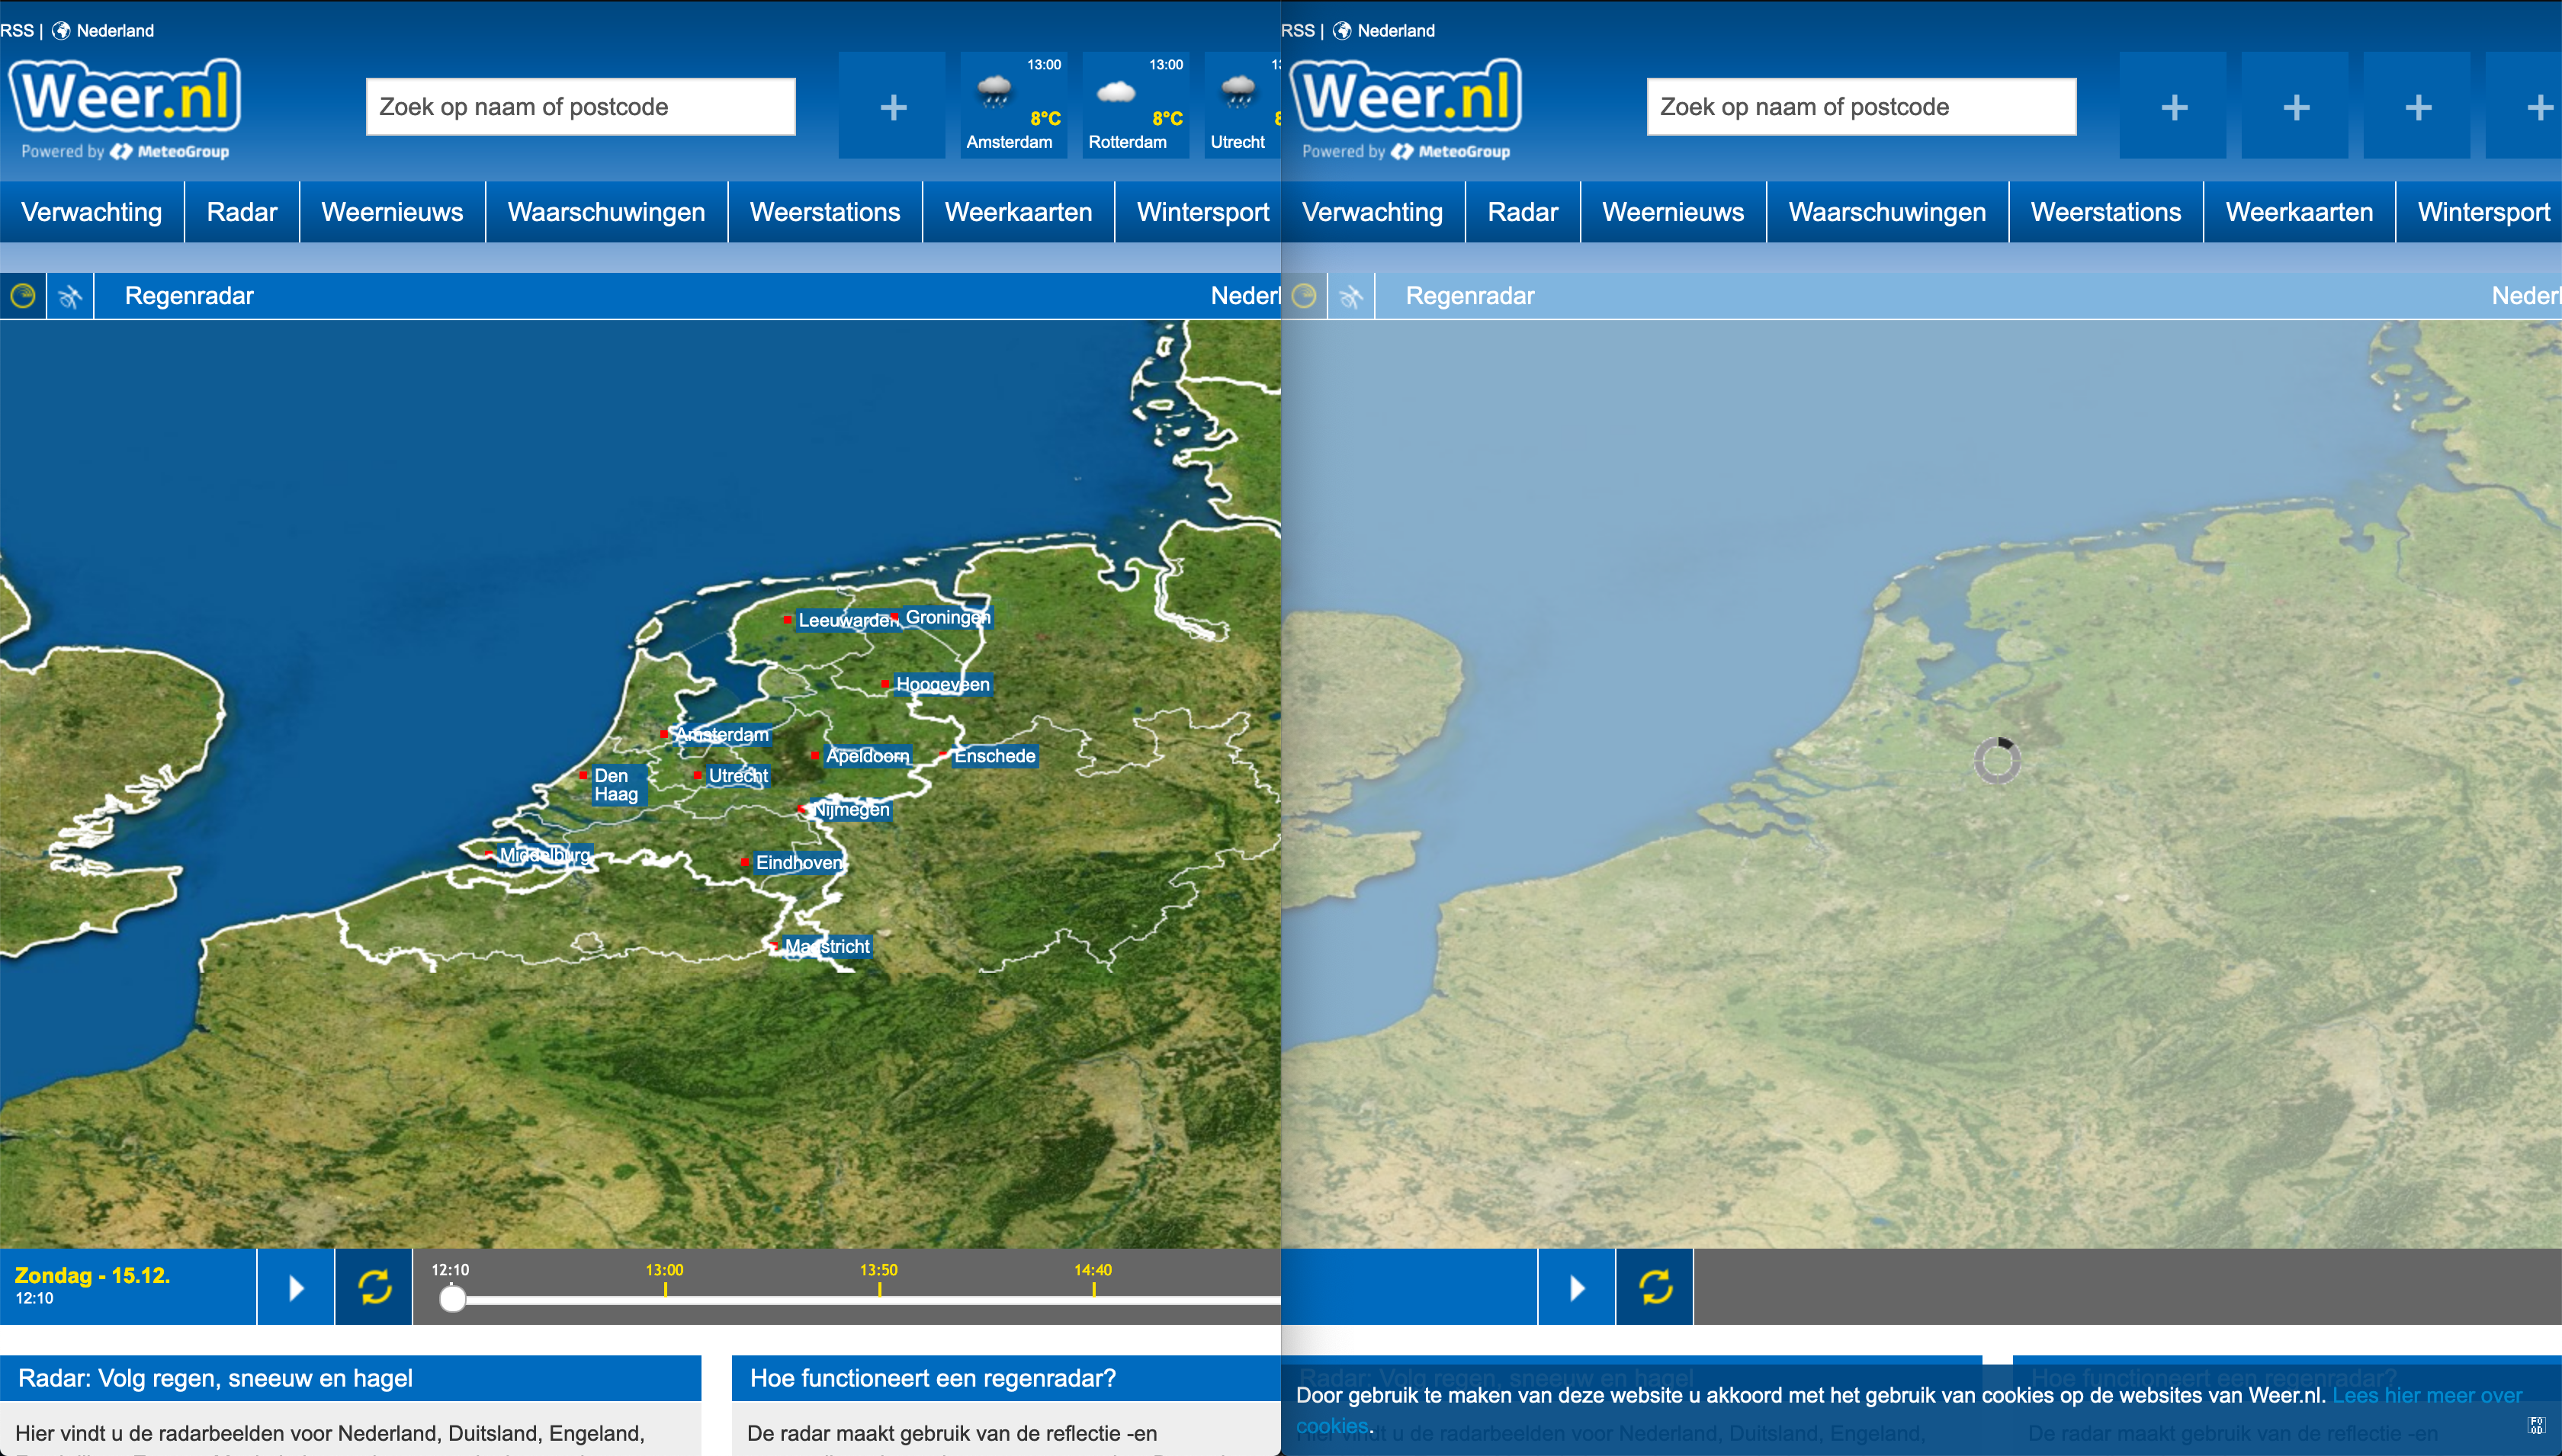
\includegraphics[width=\textwidth]{weer}

	\section{}
	The X-Cache is used to hasten the process of loading the website for the user. So instead of going to the original servers the clients request is caught by the Content Delivery Network and processed immediately.

	

	The Transfer-Encoding header specifies the form of encoding used to safely transfer the payload body to the user.

	Transfer-Encoding is a hop-by-hop header, that is applied to a message between two nodes, not to a resource itself. Each segment of a multi-node connection can use different Transfer-Encoding values. If you want to compress data over the whole connection, use the end-to-end Content-Encoding header instead.

	https://developer.mozilla.org/en-US/docs/Web/HTTP/Headers/Transfer-Encoding


	\section{}
	A cache control describes information regarding the expiration of a the resources to that page. For example the timeout for that page due to inactivity.
	

\end{document}
